%allgemeine Formatangaben
\documentclass[
 a4paper, 										% Papierformat
 12pt,												% Schriftgr��e
 ngerman, 										% f�r Umlaute, Silbentrennung etc.
 titlepage,										% es wird eine Titelseite verwendet
 bibliography=totoc,					% Literaturverzeichnis im Inhaltsverzeichnis auff�hren
 listof=totoc,								% Verzeichnisse im Inhaltsverzeichnis auff�hren
 oneside, 										% einseitiges Dokument
 captions=nooneline,					% einzeilige Gleitobjekttitel ohne Sonderbehandlung wie mehrzeilige Gleitobjekttitel behandeln
 numbers=noenddot,						% �berschriften-??Nummerierung ohne Punkt am Ende
 parskip=half									% zwischen Abs�tzen wird eine halbe Zeile eingef�gt
 ]{scrbook}


\newcommand{\titel}{Entwicklung eines Bilderkennungssystems zum finden von Duplikaten in einer Bilddatenbank bei der Registrierung neuer Bilder}
\newcommand{\abschlussart}{Bachelor of Science (B.Sc.)}
\newcommand{\arbeit}{Bachelorarbeit}
\newcommand{\hochschule}{Hochschule f�r Technik, Wirtschaft und Kultur Leipzig}
\newcommand{\fakultaet}{Fakult�t Informatik und Medien}
\newcommand{\autor}{Martino Thomann}
\newcommand{\studiengang}{Bachelorstudiengang Medieninformatik}
\newcommand{\matrikelnr}{75484}
\newcommand{\erstgutachter}{Prof. Dr. Sibylle Schwarz}
\newcommand{\zweitgutachter}{B.Sc. Marc Bellmann}
\newcommand{\ort}{Leipzig}
 			% einbinden von pers�nlichen Daten



% Anpassung an Landessprache
\usepackage[ngerman]{babel}
\usepackage{natbib}
 
% Verwenden von Sonderzeichen und Silbentrennung
\usepackage[latin1]{inputenc}	
\usepackage[T1]{fontenc}			
\usepackage{textcomp} 																% Euro-Zeichen und andere
\usepackage[babel,german=quotes]{csquotes}						% Anf�hrungszeichen
\RequirePackage[ngerman=ngerman-x-latest]{hyphsubst} 	% erweiterte Silbentrennung

% Befehle aus AMSTeX f�r mathematische Symbole z.B. \boldsymbol \mathbb
\usepackage{amsmath,amsfonts}

% Zeilenabst�nde und Seitenr�nder 
\usepackage{setspace}
\usepackage{geometry}

% Einbinden von JPG-Grafiken
\usepackage{graphicx}

% zum Umflie�en von Bildern
% Verwendung unter http://de.wikibooks.org/wiki/LaTeX-Kompendium:_Baukastensystem#textumflossene_Bilder
\usepackage{floatflt}

% Verwendung von vordefinierten Farbnamen zur Colorierung
% Palette und Verwendung unter http://kitt.cl.uzh.ch/kitt/CLinZ.CH/src/Kurse/archiv/LaTeX-Kurs-Farben.pdf
\usepackage[usenames,dvipsnames]{color} 

% Tabellen
\usepackage{array}
\usepackage{longtable}

% einfache Grafiken im Code
% Einf�hrung unter http://www.math.uni-rostock.de/~dittmer/bsp/pstricks-bsp.pdf
\usepackage{pstricks}

% Quellcodeansichten
\usepackage{verbatim}
\usepackage{moreverb} 											% f�r erweiterte Optionen der verbatim Umgebung
% Befehle und Beispiele unter http://www.ctex.org/documents/packages/verbatim/moreverb.pdf
\usepackage{listings} 											% f�r angepasste Quellcodeansichten siehe
% Kurzeinf�hrung unter http://blog.robert-kummer.de/2006/04/latex-quellcode-listing.html

% Glossar und Abbildungsverzeichnis
\usepackage[
nonumberlist, %keine Seitenzahlen anzeigen
acronym,      %ein Abk�rzungsverzeichnis erstellen
toc          %Eintr�ge im Inhaltsverzeichnis
]      %im Inhaltsverzeichnis auf section-Ebene erscheinen
{glossaries}

% verlinktes und Farblich angepasstes Inhaltsverzeichnis
\usepackage[pdftex,
colorlinks=true,
linkcolor=InterneLinkfarbe,
urlcolor=ExterneLinkfarbe]{hyperref}
\usepackage[all]{hypcap}

% URL verlinken, lange URLs umbrechen
\usepackage{url}

% sorgt daf�r, dass Leerzeichen hinter parameterlosen Makros nicht als Makroendezeichen interpretiert werden
\usepackage{xspace}

% Beschriftungen f�r Abbildungen und Tabellen
\usepackage{caption}

% Entwicklerwarnmeldungen entfernen
\usepackage{scrhack}
					% einbinden der verwendeten Latex-Pakete


\onehalfspacing 							% 1,5facher Zeilenabstand

\definecolor{InterneLinkfarbe}{rgb}{0.1,0.1,0.3} 	% Farbliche Absetzung von externen Links
\definecolor{ExterneLinkfarbe}{rgb}{0.1,0.1,0.7}	% Farbliche Absetzung von internen Links

% Einstellungen f�r Fu�noten:
\captionsetup{font=footnotesize,labelfont=sc,singlelinecheck=true,margin={5mm,5mm}}

% Stil der Quellenangabe
\bibliographystyle{alphadin}

%Ausschluss von Schusterjungen
\clubpenalty = 10000
%Ausschluss von Hurenkindern
\widowpenalty = 10000

% Befehle, die Umlaute ausgeben, f�hren zu Fehlern, wenn sie hyperref als Optionen �bergeben werden
\hypersetup{
%    pdftitle={\titel \untertitel},
%    pdfauthor={\autor},
%    pdfcreator={\autor},
%    pdfsubject={\titel \untertitel},
%    pdfkeywords={\titel \untertitel},
}

% Beispiel f�r eine Listings-Codeumbebungen
% Bei mehreren Definitionen empfielt sich das auslagern in eine externe Datei
\lstloadlanguages{Java,HTML}
\lstset{
	frame=tb,
	framesep=5pt,
	basicstyle=\footnotesize\ttfamily,
	showstringspaces=false,
	keywordstyle=\ttfamily\bfseries\color{CadetBlue},
	identifierstyle=\ttfamily,
	stringstyle=\ttfamily\color{OliveGreen},
	commentstyle=\color{GrayBlue},
	rulecolor=\color{Gray},
	xleftmargin=5pt,
	xrightmargin=5pt,
	aboveskip=\bigskipamount,
	belowskip=\bigskipamount
} 

%Den Punkt am Ende jeder Beschreibung deaktivieren
\renewcommand*{\glspostdescription}{}

% Empfehlung: Abkuerzungsverzeichnis und Glossar sind in Graduierunsarbeiten
% nicht zwingend notwendig

% %Glossar-Befehle anschalten
% \makeglossaries
% \glsenablehyper
% \input{Header/Abkuerzungen}
% \input{Header/Glossar}


\areaset[0.5cm]{16cm}{24cm}


\begin{document}

%\include{Deckblatt/titel}						% Deckblatt der vorliegenden Arbeit
% Die Daten werden in Header/Metadaten.tex eingstellt
\begin{titlepage}
\begin{Large}
\begin{center}


\includegraphics[width=0.5\textwidth]{Abbildungen/HTWK_Zusatz_de_V_Black_sRGB.png}
% \textbf{\hochschule\ \ort}\\[5pt]
% \fachbereich\\
% \studiengang\\
% \vskip 1cm
% \arbeit\\
% zur Erlangung der akademischen Grades
\\[8pt]

\arbeit\\[-1mm]
zur Erlangung des akademischen Grades\\[3mm]
\abschlussart\\[3mm]
im \studiengang\\[-1mm]
der \fakultaet%\\[-1mm]
%der \hochschule  %% kann entfallen
\\
\vfill
{\LARGE\bfseries \titel \par}
\vfill

vorgelegt von\\
 \autor%\\
% Matrikelnummer: \matrikelnr  
\\[8pt]
\ort, den \today

\end{center}
\vfill
\begin{tabular}{ll}
Erstpr�fer: & \erstgutachter\\
Zweitpr�fer: & \zweitgutachter\\
\end{tabular}
\end{Large}
\end{titlepage}

\frontmatter												% Seitenzählerstart vor dem Text


\chapter*{Zusammenfassung}
\label{sec:Zusammenfassung}
In dieser Arbeit wird der Entwurf eines Bilderkennungssystems beschrieben. 
Das System ist in der Lage  zu erkennen, ob es sich bei einem neuen Bild um Duplikat handelt, das bereits in einer Datenbank mit registrierten Bildern vorhanden ist.
Um Duplikate zu erkennen, deren Motiv im Vergleich zum Original modifiziert, aber immer noch als Kopie erkennbar sind, wird ein feature-based Bilderkennungs-Algorithmus eingesetzt. 
Innerhalb der wurden SIFT, ORB und BRIEF miteinander im Anwendungsfall von T-Shirt Designs bei Spreadshirt innerhalb von verschiedenen Szenarien getestet und miteinander verglichen.
						% Abstrakt

%% Empfehlung: Auf Danksagungen + Vorwort in wissenschaftlichen Arbeiten eher verzichten -- ggf. die entsprechenden Dateien im Ordner Inhalt anlegen und hier auskommentieren (PKW)
%% \include{Inhalt/Danksagung}					% Danksagung
%% \include{Inhalt/Vorwort}						% Vorwort

\tableofcontents										% Inhaltsverzeichnis

\mainmatter													% Seitenzählerstart Haupttext


\chapter{Einleitung}
\label{sec:Einleitung}

\section{Motivation}
\label{sec:Motivation}
Die Spread Group bietet Nutzern �ber ihre Plattformen die M�glichkeit personalisierte Produkte zu kaufen. 
Dabei k�nnen Nutzer auch eigene Designs hochladen, um diese beispielsweise auf selbst erstellten Produkten zu verkaufen. 
T�glich werden tausende solcher selbst erstellter Designs hochgeladen.
Dabei muss seitens der Spread Group sichergestellt werden, dass die hochgeladenen Designs nicht verfassungsfeindlich sind und auch nicht gegen das Urheberrecht oder die firmeninternen Nutzerrichtlinien versto�en. 
Die manuelle �berpr�fung von so vielen Designs ist sehr aufw�ndig und h�ufig kommt es vor, dass die gleichen Designs mehrmals hochgeladen werden. 
Eine automatische Sperrung, von bereits verbotenen Designs, die erneut hochgeladen werden, kann den �berpr�fungsprozess entlasten.
Daher ist ein System notwendig, dass bei neu hochgeladenen Designs Duplikate in der Datenbank der verbotenen Designs erkennen kann.

\section{Aufgabenstellung}
\label{sec:Aufgabenstellung}
Ziel dieser Bachelorarbeit ist die Entwicklung eines Systems, dass in der Lage ist, bei neuen Bildern zu erkennen, ob diese in einer Datenbank mit bereits gespeicherten Bildern auftauchen. 
Ein neues Bild soll auch dann als Duplikat erkannt werden, wenn der Bildinhalt im Vergleich zum Original transformiert, also rotiert, skaliert, verschoben oder gespiegelt wurde. 
F�lle in denen das Bild anders gef�rbt ist oder als Teil eines gr��eren Bildes auftaucht, sollen ebenfalls ber�cksichtigt werden.

Zur Implementierung des Systems soll ein feature-based (dt. merkmalbasierter) Algorithmus verwendet werden. 
Es gibt eine Vielzahl an feature-based Algorithmen, die jeweils ihre eigenen St�rken und Schw�chen haben. 
Eine Auswahl dieser Algorithmen sollen innerhalb der Arbeit f�r den Einsatz in der Bildakkreditierung bei Spread Group getestet und miteinander verglichen werden.

\section{Erfolgs- und Qualit�tskriterien}
\label{sec:ErfolgsUndQualit�tskriterien}
Die G�te des Bilderkennungssystems soll anhand von einem Testdatensatz ermittelt werden. 
Der Testdatensatz ist dabei in zwei Teils�tze unterteilt. 
Der erste Teilsatz an Bildern stellt die Menge an gespeicherten Datenbankbildern dar. 
Der zweite Teilsatz enth�lt eine Untermenge an Duplikaten aus dem Datenbanksatz und eine Menge an neuen Bildern, die nicht im Datenbanksatz auftauchen. Getestet wird in verschiedenen Szenarien, die die Robustheit des Systems gegen�ber bestimmter Sonderf�lle testen sollen. Je nach Szenario sind die Duplikate auf unterschiedliche Weise im Vergleich zum Original ver�ndert. Als Vergleich dient der pHash-Algorithmus, der momentan in der Sprad Group zur Duplikatensuche verwendet wird.

Die verwendeten Metriken werden in den Grundlagen \ref{sec:TestMetriken} erkl�rt.
Am wichtigsten ist dabei ein hoher Recall, sodass m�glichst viele Duplikate durch das System abgefangen werden. 
Da automatisch gesperrte Designs nochmal manuell gepr�ft werden, f�llt eine niedrigere Spezifizit�t bei der Auswertung nicht so sehr ins Gewicht. Laufzeit- und Speicherkosten sollen ebenfalls innerhalb der Arbeit abgesch�tzt werden. 

Um f�r die Verwendung in der SpreadGroup in Frage zu kommen, muss das neue System Duplikate zuverl�ssiger erkennen k�nnen, als die momentan eingesetzte pHash-Implementation. 
Daf�r wird ein h�herer Recall angestrebt. Um sicherzustellen, dass Spezifizit�t nicht zu sehr absinkt, wird auf eine h�here oder zumindest gleichbleibende Balancierte-Genauigkeit abgezielt.





\chapter{Grundlagen}
\label{sec:Grundlagen}
\section{feature-based Algorithmen}
\label{sec:m-based}
Ziel der feature-based (dt. Merkmalbasierten) Algorithmen ist es markante Punkte innerhalb von Bildern zu finden und zu beschreiben. Die Algorithmen bestehen dabei im Grunde aus zwei Schritten:
\begin{enumerate}
\item Schl�sselpunktsuche, bei der nach Koordinaten innerhalb eines Bildes gesucht wird, an denen sich markante Punkte befinden.
\item Erstellung von Deskriptoren, die den Bereich um die Schl�sselpunkte beschreiben. Diese sollen sp�ter mit Deskriptoren aus anderen Bildern verglichen werden, um gemeinsame Merkmale zu finden. 
\end{enumerate}

Wie genau diese beiden Schritte implementiert sind ist je nach Algorithmus unterschiedlich.

Meistens handelt es sich bei den gefundenen Merkmalen um Rand- und Eckpunkte oder Details auf einer Fl�che.
\subsection{SIFT: Scale-Invariant Feature Transform}
\label{sec:SIFT}

Ziel des SIFT-Algorithmus ist es Merkmale in einem Bild zu finden und mit Deskriptoren zu beschreiben, die Robust gegen�ber Rotation, Verschiebung und Skalierung sind. Auch der Einfluss durch Bildrauschen und Verzerrung soll m�glichst gering sein.
Dabei durchl�uft der Algorithmus 4 Schritte. Schritt 1 bis 3 umfassen die Suche und Beschreibung der Schl�sselpunkte, w�hrend Schritt 4 sich mit Erstellung der Deskriptoren befasst.  \cite[S. 2]{sift1999} 

\paragraph{1. Suche nach Extrempunkten}
\label{sec:Extrempunktsuche}

SIFT sucht nach Extrempunkten innerhalb von Bildern. Extrempunkte sind dabei Punkte, an denen lokale Maxima oder Minima in der Helligkeit auftreten. Also helle Punkte innerhalb von dunklen Bereichen und dunkle Punkte innerhalb von hellen Bereichen. 

Um Extrempunkte zu finden wird der "Difference of Gaussian" genutzt. Zuerst wird eine bestimmte Anzahl an Bildern, durch das Weichzeichnen des Originalbilds mit dem Gauschen Weichzeichner, erstellt. 
Der Grad der Unsch�rfe steigt dabei bei jedem Bild um einen konstanten Faktor. Ein Satz dieser weichgezeichneten Bilder wird  als Oktave bezeichnet. 
F�r jedes paar an aneinander grenzenden weichgezeichneten Bildern, wird die Differenz berechnet. Bei dieser Differenz handelt es sich um den "Difference of Gaussian". Durch den "Difference of Gaussian" werden Rand- und Eckpunkte, sowie andere Details im Bild hervorgehoben.
Bei der Implementation von SIFT werden pro Oktave meist f�nf weichgezeichnete Bilder verwendet, aus denen vier "Difference of Gaussian" Bilder entstehen. \cite[S. 94]{sift2004}

Jeder Pixel der mittleren "Difference of Gaussian" Bilder wird mit seinen acht Nachbarn innerhalb desselben Bildes und seinen je neun Nachbarn im DOG dar�ber und darunter verglichen. 
Ein Pixel ist dann ein Schl�sselpunkt, wenn sein Helligkeitswert gr��er oder kleiner als der Wert all seiner Nachbarn ist. \cite[S. 95]{sift2004}

Diese Extrempunktsuche wird dabei f�r mehrere Oktaven durchgef�hrt. Dabei wird f�r jede Oktave das Originalbild um den Faktor 2 herunter skaliert. 
Das ist notwendig, da manche Extrempunkte nur bei bestimmten Aufl�sungen auffindbar sind. \cite[S. 94f]{sift2004}
Durch die Sammlung von Schl�sselpunkten auf verschiedenen Aufl�sungen, sind diese bei Bildern in verschiedenen Aufl�sungen vergleichbar. Der Aufbau von "Difference of Gaussian" Bilder innerhalb von mehreren Oktaven wird als scale-space (dt. Bildpyramide) bezeichnet.

\paragraph{2. Akkurate Ortsbestimmung der Schl�sselpunkte} 

Die Positionen der Schl�sselpunkte, die auf niedrigen Aufl�sungen gefunden wurden, entspricht gegebenenfalls nicht genau der Position in der Originalaufl�sung. 
Deshalb wird die Taylorreihe verwendet, um die tats�chliche Position zu interpolieren. \cite[S. 97f]{sift2004}

Au�erdem werden Schl�sselpunkte an R�ndern und Schl�sselpunkte mit niedrigem Kontrast zu ihrer Umgebung herausgefiltert. Das ist n�tig, da solche Schl�sselpunkte Deskriptoren hervorbringen, die nicht zuverl�ssig verglichen werden k�nnen. \cite[98f]{sift2004}

\paragraph{3. Bestimmung der Schl�sselpunkt Ausrichtung}
\label{sec:SchluesselpunktOrienierung}

Um Schl�sselpunkte und die aus ihnen resultierenden Deskriptoren robust gegen�ber Bildrotationen zu machen, wird jedem Schl�sselpunkt eine Ausrichtung zugewiesen. 
Damit diese Ausrichtung konsistent ist, wird diese anhand der lokalen Bildeigenschaften um den Schl�sselpunkt herum bestimmt. \cite[S. 99]{sift2004}

Um das zu erreichen, wird ein 360 Grad umfassendes Histogramm mit 36 bins aufgebaut. Anhand der Skalierung des Schl�sselpunkts wird ein weichgezeichnetes Bild mit passender Skalierung gew�hlt. 
Innerhalb dieses Bildes werden Abtastpunkte um den Schl�sselpunkt herum genommen. F�r jeden Abtastpunkt wird die Orientierung und St�rke des Gradienten bestimmt. 
Der Gradient beschreibt dabei die �nderung der Pixelhelligkeit innerhalb eines Bildes. 
Sowohl St�rke als auch Orientierung des Gradienten sind f�r alle Ebenen der Bildpyramide vorberechnet worden. \cite[S. 99]{sift2004}

Jede Gradient-Orientierung wird in das Histogramm eingetragen und anhand der Gradient-St�rke gewichtet. Da das Histogramm 36 bins hat, werden Orientierungen in 10-Grad-Schritten zusammengefasst. Aus dem Histogramm wird die Orientierung des globalen Maximums, sowie die Orientierungen aller lokalen Maxima die mindestens 80 Prozent des globalen Maximums betragen, entnommen. F�r jede entnommene Orientierung wird ein Schl�sselpunkt erstellt. Dadurch kann es mehrere Schl�sselpunkte mit der gleicher Position und Skalierung aber mit unterschiedlichen Orientierungen geben. \cite[S. 100]{sift2004}

\paragraph{4. Deskriptoren erstellen} 

In dem Bereich um den Schl�sselpunkt werden wie im Schritt 3 (Abschnitt ~\ref{sec:SchluesselpunktOrienierung}) f�r jeden Abtastpunkt die Gradienten-St�rke und -Orientierung bestimmt. Der Bereich wird dabei in 4x4 gro�e Unterbereiche aufgeteilt, f�r die ein Histogramm erstellt wird. Dabei werden f�r das Histogramm nur 8 bins verwendet, in denen Gradienten-St�rken mit �hnlicher Orientierung aufsummiert werden. Aus diesen Werten wird ein Deskriptor erstellt. �blicherweise werden Abtastbereiche mit einer Gr��e von 16x16 verwendet. Daraus ergeben sich insgesamt 16 Unterbereiche der Gr��e 4x4 mit je 8 Orientierungs-bins. Ein typischer Deskriptor ist ein Vektor mit 16 * 8 = 128 Werten. \cite[S. 101]{sift2004}

\subsection{ORB: Oriented FAST and Rotated BRIEF}
\label{sec:ORB}
ORB basiert auf dem FAST-Algorithmus f�r die Schl�sselpunktsuche und dem BRIEF-Algorithmus f�r die Generierung von Deskriptoren

\paragraph{Sch�sselpunktsuche mit FAST}
\label{sec:FAST}

Der FAST-Algorithmus sucht nach Eckpunkten in einem Bild. Dazu wird um jeden Pixel im Bild ein Kreis mit 16 Randpixeln gezogen. Der betrachtete Kandidat-Pixel ist genau dann ein Eckpunkt, wenn eine bestimmte Anzahl an aneinander grenzenden Randpixel heller oder dunkler sind als der Kandidat-Pixel plus oder minus einem bestimmten Schwellenwert. \cite[S. 4]{fast2006}

\begin{figure}[h]
\centering
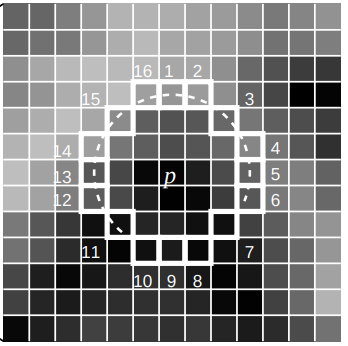
\includegraphics[scale=.7]{Abbildungen/fast}
\caption{Randpixel um Kandidat-Pixel aus \cite[S. 4]{fast2006}}
\label{fig:pixelkreis}
\end{figure}

Bei der Implementation in ORB m�ssen 9 der 16 Randpunkte heller oder dunkler als der Kandidat-Pixel sein, damit dieser sich als Randpunkt qualifiziert. 
Zudem wird die "Harris corner measure" genutzt, um Randpunkte herauszufiltern. 
Dazu wird jedem Schl�sselpunkt ein Wert zugeteilt, der aussagt, wie wahrscheinlich es ist, dass es sich bei dem Schl�sselpunkt um einen Eckpunkt handelt. Der Schwellenwert, um sich als Eckpunkt zu qualifizieren, wird niedrig genug gesetzt um eine bestimmte Mindestanzahl an Schl�sselpunkten zu erreichen. 
Die Mindestanzahl an Schl�sselpunkten, kann dabei je nach Anwendungsfall variieren. Es muss gen�gend Schl�sselpunkte geben, um das Bild zu beschreiben. 
Gleichzeitig m�chte man aber Schl�sselpunkte vermeiden deren Deskriptoren nicht zuverl�ssig verglichen werden k�nnen. \cite[S. 2565]{orb2011}

Die durch FAST gefundenen Schl�sselpunkte sind anders als bei SIFT noch nicht Robust gegen�ber Rotations- und Aufl�sungsunterschieden. 
Um Invarianz gegen�ber Aufl�sungsunterschieden entgegenzuwirken, generiert ORB mehrere niedriger aufgel�ste Varianten des Originalbilds. 
F�r jede Aufl�sung wird die Schl�sselpunktsuche mit FAST und Randpunktfilterung mit "Harris corner measure" durchgef�hrt. 
Um die Orientierung des Schl�sselpunkts zu ermitteln, wird in dessen Umgebung nach dem Pixel mit dem h�chsten Helligkeitswert gesucht. Die Orientierung ergibt sich dann aus dem Vektor zwischen diesen beiden Punkten. \cite[S. 2565]{orb2011} 

\paragraph{Erstellen der Deskriptoren mit BRIEF} Der BRIEF-Algorithmus definiert um den Schl�sselpunkt einen Bereich $p$, der weichgezeichnet wird. 
Aus diesem Bereich werden $n$ Pixelpaare $(x,y)$ genommen und einem Bin�rtest $\tau$ unterzogen. F�r jedes Pixelpaar werden die Helligkeitswerte $p(x)$ und $p(y)$ verglichen. 
Je nachdem ob der Helligkeitswert $p(x)$ gr��er als $p(y)$ ist, ergibt der Bin�rtest $\tau$ 0 oder 1. In der Implementation bei ORB werden 256 Pixelpaare genutzt.  
Der Deskriptor ist eine Aneinanderreihung der Testergebnisse aller 256 Pixelpaare. Somit ergibt sich ein 256 Bit Deskriptor pro gefundenen Schl�sselpunkt. \cite[S. 2566]{orb2011}

$$\tau (p; x, y) := \left\{
\begin{array}{ll}
1 & :p(x) < p(y) \\
0 & :p(x) \geq p(y) \\
\end{array}
\right. $$

$$f_n(p) := \sum_{1 \leq i \leq n} 2^{i-1} \tau(p; x_i, y_i) $$

Damit die durch BRIEF erstellten Deskriptoren robust gegen�ber Rotationen sind, nutzt ORB die Orientierung, die f�r die Schl�sselpunkte ermittelt wurden. 
Dazu wird eine Matrix $S$ mit den Pixelpaaren f�r den Bin�rtest erstellt. 
Gem�� der Orientierung $\theta$ des Schl�sselpunkts wird eine Rotationsmatrix $ R_\theta$ erstellt. Matrix $S$ wird mit der Rotationsmatrix $ R_\theta$ rotiert und ergibt $S_\theta$. 
Der Deskriptor f�r den Schl�sselpunkt wird anhand der rotierten Pixelpaare aus $S_\theta$ erstellt. \cite[S. 2566]{orb2011}

$$ g_n (p, \theta) := f_n(p) | (x_i, y_i) \in S_\theta$$


 
\subsection{BRISK: Binary Robust Invariant Scalable Keypoints}
\label{sec:BRISK}

\paragraph{Schl�sselpunktsuche}
�hnlich wie in SIFT wird bei BRISK eine Bildpyramide mit Oktaven aufgebaut. 
Auch hier wird die Aufl�sung jeder folgenden Oktave halbiert.
Allerdings werden, anders als bei SIFT, keine weichgezeichneten Varianten zur Berechnung des DOG in den einzelnen Oktaven erstellt.  
Stattdessen besteht jede Oktave aus einen einzelnen Bild und es werden Intra-Oktaven zwischen den Oktaven berechnet. �blicherweise werden 4 Oktaven und 4 Intra-Oktaven genutzt. \cite[S.2549]{brisk2011}  

\begin{figure}[h]
\centering
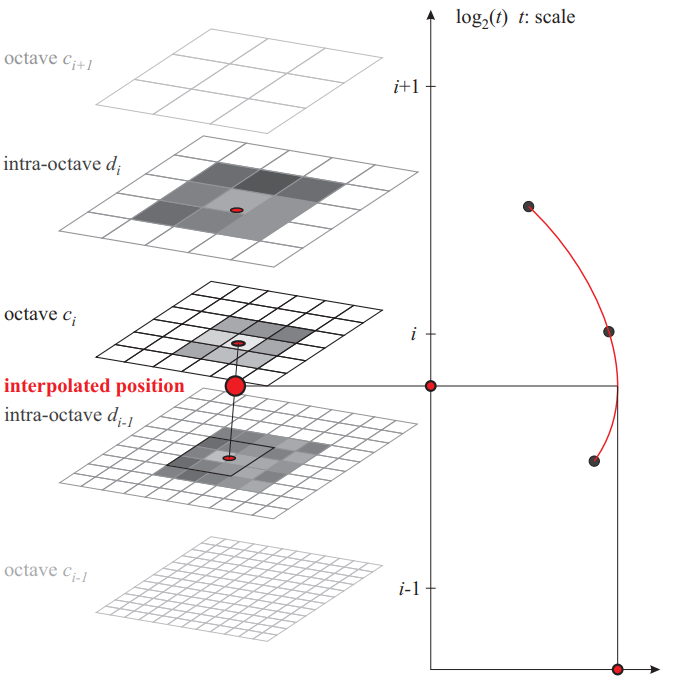
\includegraphics[scale=.4]{Abbildungen/bildpyramidebrisk}
\caption{Interpolation der Schl�sselpunktaufl�sung in der Bildpyramide aus \cite[S. 2550]{brisk2011}}
\label{fig:BildpyramideBRISK}
\end{figure}

Die erste Intra-Oktave wird erstellt, indem die Aufl�sung des Originalbilds um den Faktor 1.5 reduziert wird. 
Die Aufl�sung der ersten Intra-Oktave betr�gt dann also 2/3 der Aufl�sung des Originalbilds.
Alle weiteren Intra-Oktaven leiten sich aus der ersten ab, indem die Aufl�sung f�r alle weiteren Intra-Oktaven halbiert wird.
Ziel der Bildpyramide ist es, genau wie bei SIFT, durch Suchen auf verschiedenen Aufl�sungsebenen Schl�sselpunkte zu finden und Deskriptoren zu berechnen, die Robust gegen�ber �nderungen in der Aufl�sung sind. \cite[S.2549f]{brisk2011}  

BRISK nutzt AGAST f�r die Implementierung der Schl�sselpunktsuche. \cite[S. 2552]{brisk2011} 
AGAST ist ein Algorithmus zum finden von Eckpunkten, der �hnlich wie FAST (siehe Abschnitt \ref{sec:FAST}) funktioniert.
F�r jede Oktave und Intra-Oktave wird AGAST angewendet um potenzielle Schl�sselpunkte zu finden.
Danach wird f�r den Schl�sselpunktpixel, sowie allen 8 benachbarten Pixeln der \textit{saliency-score} berechnet.
Dieser score gibt an f�r welchen maximalen Schwellenwert sich der Pixel noch als Eckpunkt qualifiziert.
Der \textit{saliency-scores} muss f�r den Schl�sselpunkt-Kandidaten gr��er sein als der all seiner Nachbarn.
Danach werden auch die scores in dem gleichen Bereich f�r die beiden angrenzenden (Intra-)Oktaven berechnet.
Anhand der drei \textit{saliency-scores}, die in der Regel unterschiedliche Werte haben, wird eine Parabel gebaut. Das Ziel ist, mithilfe der Parabel, die Aufl�sungsebene zu interpolieren, in der der Schl�sselpunkt den h�chsten \textit{saliency-score} erreicht. Diese Aufl�sungsebene, kann sich dabei zwischen den Oktaven befinden.
Dadurch erh�lt man, die Position und die Skalierung, des Schl�sselpunkts. \cite[S. 2550]{brisk2011}

\paragraph{Erstellen des Deskriptors}
BRISK nutzt ein vordefiniertes Muster, um Positionen f�r Abtastpunkte zu definieren.
Die Abtastpunkte sind in konzentrischen Kreisen um den Schl�sselpunkt herum positioniert.
Auf die Bereiche um die Abtastpunkte herum wird der Gau�sche Weichzeichner angewendet.
Au�erdem wird das Muster an die Position und Skalierung des Schl�sselpunkts angepasst.
Insgesamt werden 60 Abtastpunkte definiert, die miteinander gepaart werden.\cite[S. 2551]{brisk2011}

\begin{figure}[h]
\centering
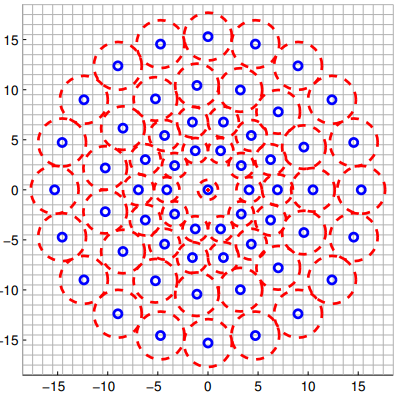
\includegraphics[scale=.5]{Abbildungen/abtastmusterbrisk}
\caption{Vordefiniertes Abtastmuster mit Abtastpunkten in blau und weichgezeichnete Bereiche in rot aus \cite[S. 2551]{brisk2011}}
\label{fig:abtastmuster}
\end{figure}


Abh�ngig von der Skalierung des Schl�sselpunkts werden Schwellenwert-Distanzen bestimmt, mit denen die Paare in Langdistanzpaare $L$ und Kurzdistanzpaare $S$ unterschiedenen werden. Um die Orientierung des Schl�sselpunkts zu ermitteln wird folgende Formel auf die Langdistanzpaare angewendet:

$$\begin{pmatrix}
	g_x \\
	g_y \\
\end{pmatrix}
= \frac{1}{|L|} * \sum_{(p_i,p_j) \in L} \textbf{g}(p_i, p_j)$$

$\textbf{g}(p_i,p_j)$ ist dabei der Gradient der Helligkeitswerte zwischen der Abtastpunkten $p_i$ und $p_j$ einer Paarung. Der Winkel ergibt sich dann aus $\alpha = arctan2(g_y,g_x)$. Es werden nur die Langdistanzpaarungen f�r die Berechnung der Orientierung verwendet, da davon ausgegangen wird, dass sich die Gradienten der Kurzdistanzpaarungen gegenseitig aufheben w�rden. \cite[S. 2551]{brisk2011}

Damit der Deskriptor Robust gegen�ber Rotationen ist, wird das Abtastmuster mit den Winkel $\alpha$ um den Schl�sselpunkt rotiert. 
Um den Deskriptor zu erstellen werden f�r alle Kurdistanzpaarungen auf dem rotierten Abtastmuster die Helligkeitswerte der beiden Abtastpunkte miteinander verglichen.
Je nachdem welcher Helligkeitswert gr��er ist, wird ein Bit in einer Bitfolge auf 0 oder 1 gesetzt. 
Diese Bitfolge stellt den Deskriptor f�r BRISK dar. Insgesamt hat die Bitfolge 512 Stellen, woraus sich ein 512 Bit Deskriptor f�r jeden Schl�sselpunkt ergibt. \cite[S. 2551]{brisk2011}

\section{Match-Suche mit Deskriptoren}
\label{sec:Matching}

Im Abschnitt  ~\ref{sec:m-based} wurden die Merkmalbasierten-Algorithmen erkl�rt, mit denen Deskriptoren f�r Merkmale in einem Bild generiert werden k�nnen.
In diesem Abschnitt soll es darum gehen, wie diese Deskriptoren genutzt werden k�nnen, um die Merkmale aus zwei Bildern zu vergleichen und �bereinstimmungen zu finden. �bereinstimmungen werden auch als Match bezeichnet.

\subsection{Deskriptoren Vergleichen}
\label{sec:DeskriptorenVergleichen}

Um zwei Deskriptoren zu vergleichen, wird die Distanz zwischen den beiden berechnet. 
Die Distanz beschreibt in diesem Fall wie �hnlich sich Deskriptoren sind. 
Je kleiner die Distanz desto �hnlicher die Deskriptoren.
Abh�ngig davon welche Art Deskriptor verglichen wird, wird ein anderer Distanzma�stab verwendet.

\paragraph{Euklidische-Distanz}
Bei Deskriptoren, die aus dem SIFT-Algorithmus resultieren, wird die Euklidische Distanz genutzt. \cite[S. 104]{sift2004} Die Deskriptoren sind hierbei eine Folge von Gradient-Werten. 
Stelle f�r Stelle wird die Euklidische Distanz f�r alle Gradient-Werte der Deskriptoren berechnet und aufsummiert. 

$$distance(desc1, desc2) := \sum_{ i = 1 }^{ 128 }{ \sqrt{ (desc1[i] - desc2[i])^2 } }$$

SIFT-Deskriptoren bestehen in der Regel aus 128 Gradient-Werten.

\paragraph{Hamming-Distanz}
Die Hamming-Distanz kann verwendet werden, um Bitfolgen zu vergleichen. 
Dazu werden beide Bitfolgen Stelle f�r Stelle verglichen. 
F�r jede Stelle, die nicht �bereinstimmt, steigt die Distanz um 1.

$$distance(desc1, desc2) := \vert \{ i \in \{1,..., 256\} \mid desc1_{i} \neq desc2_{i}\} \vert$$

Die Hamming-Distanz eignet sich um Deskriptoren, die durch den ORB- oder BRISK-Algorithmus errechnet werden, zu vergleichen. \cite[S.  2569]{orb2011} 
Bei diesen handelt es sich um Bitfolgen mit 256 Stellen bei ORB und 512 Stellen bei BRISK. Auch bei dem Vergleich von pHash-Werten kommt die Hamming-Distanz zum Einsatz. 

Durch bitweises XOR kann die Hamming-Distanz deutlich effizienter berechnet werden, als die Euklidische Distanz. 
Bin�r-Deskriptoren haben dadurch beim Vergleichen einen Geschwindigkeitsvorteil.

\subsection{Matching Strategien}
\label{sec:MatchingStrategien}

\paragraph{Brute-Force Matcher}
\label{sec:BFM}
Um �bereinstimmungen von Merkmalen in zwei Bildern zu finden, werden alle Deskriptoren des ersten Bilds mit allen Deskriptoren des zweiten Bilds verglichen. \cite{opencv}

Der Vorteil dieser simplen Herangehensweise ist, dass garantiert die besten Matches gefunden werden. 
Allerdings ist diese Strategie mit $\mathcal{O}(n^2)$ auch sehr ineffizient, wodurch sie gerade bei Datensets mit einer gro�en Menge an Deskriptoren ins Gewicht f�llt. 

\paragraph{FLANN-Based Matcher}
FLANN ist eine Bibliothek f�r fast approximate nearest neighbor search. 
Abh�ngig vom verwendeten Datensatz w�hlt die Bibliothek automatisch aus einer Reihe von Algorithmen, die f�r approximate nearest neighbor Suche optimiert sind, den besten aus. F�r gr��ere Datensets arbeitet FLANN schneller als der Brute-Force Matcher. Allerdings kann durch die approximate nearest neighbor search nicht garantiert werden, dass FLANN die besten Matches findet. \cite{opencv}


\subsection{Filterung der Matching-Ergebnisse}
\label{sec:RatioTest}
F�r jeden Deskriptor aus dem ersten Bild wird der  erst- und zweitbeste Match aus dem zweiten Bild gespeichert. Ein Match besteht dabei aus den beiden Deskriptoren, die verglichen werden, und die resultierende Distanz (Siehe Abschnit ~\ref{sec:DeskriptorenVergleichen}). Daraus ergibt sich eine 2xN Matrix, wobei N die Anzahl der Deskriptoren im ersten Bild darstellt.

Es k�nnen Deskriptoren vorkommen, f�r die keine zuverl�ssiger Match gefunden werden kann. Das kann unter anderen passieren, wenn Schl�sselpunkte an R�ndern von Objekten oder wirren Bereichen im Bild gefunden werden. 
Weil mit solchen Deskriptoren keine gute Aussage �ber die �hnlichkeit von zwei Bildern getroffen werden kann, m�ssen diese herausgefiltert werden.

Dazu schl�gt Lowe den sogenannten "ratio test" vor. 
Dabei wird die Distanz des erst- und zweitbesten Matchs verglichen. Wenn das Verh�ltnis zwischen den beiden Distanzen kleiner als 0.8 ist, wird der erstbeste Match behalten. 
Ansonsten wird der Match verworfen.
Dieses Vorgehen basiert auf der Annahme, dass die Distanz beim erstbesten Match deutlich niedriger als die Distanz beim zweitbesten Match sein muss, damit der erstbeste Match als zuverl�ssig gilt. 
Sind die Distanzen zu �hnlich, kann kein eindeutiger Match f�r den Deskriptor gefunden werden. \cite[S.104]{sift2004}



\section{Test-Metriken}
\label{sec:TestMetriken}
Das Bilderkennungssystem soll die Bilder in zwei Klassen einordnet: Duplikate und Unikate. 
Da es in diesem Fall bei der Klassifizierung nur zwei m�gliche Klassen gibt, kann man das Bilderkennungssystem als bin�ren Klassifikator bezeichnen. 

Die Performance von bin�ren Klassifikatoren kann durch die Werte einer Wahrheitsmatrix quantifiziert werden. 
Die Wahrheitsmatrix gibt dabei an, wie viele richtige und falsche Entscheidungen das System bei der Klassifikation getroffen hat. \cite[S. 170]{classification}
\begin{table}[h]
\begin{tabular}[h]{ l | l | l}
&Duplikat&Unikat \\
System Klass.:&&\\
\hline
Duplikat&Anzahl richtige Duplikate (TP) &Anzahl falsche Duplikate (FP) \\
\hline
Unikat&Anzahl falsche Unikate (FN) &Anzahl richtige Unikate (TN)
\end{tabular}
\caption{Wahrheitsmatrix f�r Duplikaten-Suche}
\label{Wahrheitsmatrix f�r Duplikaten-Suche}
\end{table}

Aus den Werten der Wahrheitsmatrix lassen sich weitere Metriken ableiten, die f�r die Bewertung eines bin�ren Klassifikators n�tzlich sein k�nnen. Interessant f�r diese Arbeit sind Recall, Spezifizit�t und Balancierte-Genauigkeit.

Der Recall, oder auch true positive rate, gibt das Verh�ltnis zwischen den Duplikaten, die das System korrekt klassifiziert hat, und allen Duplikaten, die sich in dem Suchdatensatz befinden, an. \cite[S. 172]{classification}

$$Recall = \frac{ TP }{ TP + FN }$$

Die Spezifizit�t, oder auch true negative rate, gibt das Verh�ltnis zwischen den Unikaten, die das System korrekt klassifiziert hat, und allen Unikaten, die sich im Suchdatensatz befinden an. \cite[S. 172]{classification}

$$Specificity = \frac{ TN }{ FP + TN }$$

Die Accuracy (dt. Genauigkeit), gibt das Verh�ltnis zwischen den Bildern, die das System korrekt klassifiziert hat, und allen Bildern im Suchdatensatz an.
Sie spiegelt die F�higkeit des Systems Bilder richtig zu Klassifizieren wieder. \cite[S. 171]{classification}

$$Accuracy = \frac{ TP + TN }{ TP + TN + FP + FN } = \frac{ Recall * P + Specificity * N }{ P + N }$$

Allerdings ist die Genauigkeit kein zuverl�ssiger Wert, wenn man mit unausgeglichenen Datens�tzen arbeitet. 
Ein Datensatz gilt dann als unausgeglichen, wenn einer Klassifikation mehr Elemente angeh�ren, als der anderen Klassifikation. \cite[S. 171]{classification}
In den Testdatens�tzen, die f�r diese Arbeit verwendet werden, befinden sich mehr Unikate als Duplikate.
Dieses Ungleichgewicht kann die Genauigkeit stark beeinflussen. So kann zum Beispiel eine gute Spezifizit�t einen schlechten Recall ausgleichen, wenn der Datensatz zum gr��ten Teil aus Unikaten besteht.

Daher kommt bei unbalancierten Datens�tzen die balanced-accuracy (dt. Balancierte-Genauigkeit) zum Einsatz. \cite[S. 175]{classification} 

$$Balanced-Accuracy = \frac{ Recall + Specificity }{ 2 }$$

Da sie den Durchschnitt aus Recall und Spezifizit�t bildet, werden Unterschiede zwischen den beiden Werten ausgeglichen. Dadurch ist die Balancierte-Genauigkeit robust gegen�ber unausgeglichenen Datens�tzen.


\chapter{Analyse}
\label{sec:Analyse}
\section{Duplikate}
\label{sec:Duplikate}

\paragraph{Definition}
Im Kontext dieser Arbeit sind mit Duplikaten Bilder gemeint, die den gleichen Inhalt wie ein bereits bekanntes Bild haben. 
Der Inhalt ist in diesem Fall im optischen und nicht im semantischen Sinne gemeint. Ein Duplikat muss optische gleiche, oder zumindest sehr �hnliche Merkmale im Vergleich zum Original aufweisen. 
Wenn zwei Bilder ein Haus zeigen, und somit im semantischen Sinne den gleichen Inhalt haben, ist das erstmal nicht interessant. 
Nur wenn die H�user �hnliche oder gleiche Merkmale aufweisen, indem sie zum Beispiel den gleichen Aufbau haben, kommt eine Klassifizierung als Duplikat in Frage.

Da der Vergleich von Merkmalen hierbei eine zentrale Rolle spielt, muss ein Bild keine pixelgenaue Kopie sein um als Duplikat zu gelten.
Ein Bild kann auch dann ein Duplikat sein, wenn sein Inhalt im Vergleich zum Original rotiert, skaliert, verschoben oder gespiegelt wurde.
Bilder mit anderer Hintergrundfarbe und anders gef�rbten Motiv k�nnen ebenfalls als Duplikat gelten. 
Wichtig ist, die Form der Merkmale.
Auch wenn das Motiv des Originalbilds als Teil des Motivs, des neuen Bilds auftaucht, soll es im Sinne der Arbeit als Duplikat erkannt werden.

Diese sehr weit gefasste Definition von Duplikaten ist n�tig, damit die Bildakkreditierung der Spread Group nicht so einfach �berlistet werden kann. 
Der Nutzer soll nicht in der Lage sein, auf Plattformen der Spread Group ein verbotenes Bild hochzuladen, wenn er es �ber die genannten Methoden ver�ndert. 
Ein Bild wird aufgrund seines Inhalts verboten. Solange der verbotene Inhalt erkennbar ist, spielt es keine Rolle, wie er transformiert wurde.

\paragraph{Duplikate mit Merkmalen erkennen}
Die in den Grundlagen in Abschnitt ~\ref{sec:Grundlagen} vorgestellten merkmalbasierten Algorithmen liefern Deskriptoren. 
Wenn zwei Bilder verglichen werden, kann mit den Deskriptoren nach �bereinstimmungen, auch Matches genannt, gesucht werden. 

Die Menge an gefundenen Matches an sich gibt allerdings noch keinen Aufschluss dar�ber, ob die beiden Bilder tats�chlich �bereinstimmen. 
Es braucht eine Formel, die anhand der Matches eine Aussage dar�ber treffen kann, wie �hnlich sich zwei Bilder sind.
Bei meiner Recherche habe ich keine konkrete Formel gefunden, die das bewerkstelligt.
Daher muss eine eigene Formel entwickelt werden.
\section{Baseline-Algorithmus (pHash)}
\label{sec:pHash}
Spreadshirt nutzt momentan einen Perceptual-Hashing-Algorithmus (kurz pHash) um neu hochgeladene Bilder zu erkennen, die bereits verboten wurden. Die Idee von pHash ist, dass f�r �hnliche Bilder ein �hnlicher pHash-Wert ermittelt wird. Die pHash Implementierung bei Spreadshirt st�tzt sich auf den Blockeintrag \cite{pHash} und l�sst sich grob in drei Phasen unterteilen.

\paragraph{Phase 1: Vorverarbeitungsphase}
Zuerst kommt das Bild in eine Vorverarbeitungsphase. Falls das Bild einen transparenten Hintergrund hat, wird es so zugeschnitten, dass der Bildrand direkt Rand des Motivs liegt. Danach wird das Bild auf eine Aufl�sung von 32x32 herunter skaliert und in ein Graustufenbild umgewandelt. 

\paragraph{Phase 2: Umwandlung in den Frequenzraum} In dieser Phase wird das Bild vom Ortsraum in den Frequenzraum �berf�hrt. 
Dazu wird die diskrete Kosinustransformation genutzt. 
Es entsteht eine 32x32 DCT-Matrix bestehend aus Koeffizienten, mit denen, in Kombination mit der Kosinusfunktion, das Originalbild rekonstruiert werden kann. 

F�r pHash wird der obere linke 8x8 Bereich der DCT-Matrix genutzt. Dieser Bereich enth�lt die Niederfrequenzkomponenten und wird als reduzierte DCT-Matrix bezeichnet.  
Die Niederfrequenzkomponenten sind f�r pHash interessant, da diese die groben Strukturen und Muster des Bilds beschreiben. Zwei Bilder mit �hnlichen Strukturen und Mustern werden �hnliche Niederfrequenzkomponenten haben und damit zu �hnlichen Hash-Werten f�hren. 

\paragraph{Phase 3: Hash-Berechnung}
F�r die Hash-Berechnung wird der Median in der reduzierten DCT-Matrix ermittelt. Die reduzierte DCT-Matrix der Gr��e 8x8 beinhaltet insgesamt 64 Werte. F�r jeden Wert wird gepr�ft, ob er �ber oder unter dem Median liegt. 
Wenn der Wert gr��er ist, wird eine 1 und ansonsten eine 0 an den Hash-Wert angeh�ngt. Damit ergibt sich ein 64-bit Hash-Wert f�r ein Bild.

\paragraph{pHash-Werte vergleichen}
Zum vergleichen von pHash-Werten, wird die Hamming-Distanz (Siehe Abschnitt ~\ref{sec:DeskriptorenVergleichen}) genutzt.
Bei Spreadshirt gilt ein Bild als Duplikat, wenn beim Hash-Vergleich mit einem Bild aus der Datenbank eine Hamming-Distanz kleiner oder gleich 4 ermittelt wird.


\section{Test-Daten}
\label{sec:TestDaten}

Um die Algorithmen auf ihre Leistung im Anwendungsfall bei Spreadshirt testen zu k�nnen, sind Bilder notwendig, die repr�sentativ f�r die Designs, die bei Spreadshirt hochgeladen werden, sind. 

F�r die Tests werden die Datens�tze f�r jedes Szenario erstellt (siehe Abschnitt ~\ref{sec:TestSzenarien} und in zwei Subsets geteilt:

\begin{itemize}
\item \textbf{Datenbank-Set} 
Bilder, die in der Datenbank registriert werden.

\item \textbf{Such-Set}
Suchbilder, die mit den Bildern aus der Datenbank verglichen werden sollen. 
Das Set enth�lt dabei Duplikate aus dem Datenbank-Set, die entsprechend des Szenarios modifiziert sind.  
Es sind auch Bilder enthalten, die keine Duplikate aus dem Datenbank-Set sind und auch nicht als solche erkannt werden sollen. 
\end{itemize}


\section{Vorgehen}
\label{sec:Vorgehen}

Aus der Betrachtung der Problemstellung ergeben sich die folgenden Teilaufgaben:

\begin{enumerate}
\item Definition einer Formel zur Bestimmung der �hnlichkeit von zwei Bildern
\item Evaluation des Baseline-Algorithmus und der merkmalbasierten Algorithmen
\begin{enumerate}
\item Definition von Test-Szenarien in denen die Algorithmen verglichen werden
\item Erstellung von Testbildern f�r Test-Szenarien
\item Entwicklung eines Test-Systems, das die Algorithmen durch die Test-Szenarien laufen l�sst und Statistiken festh�lt
\item Auswertung der Tests zur Evaluation des Baseline-Algorithmus und zur Bestimmung welcher Feature-Based Algorithmus am besten f�r das neue Bilderkennungssystem geeignet ist
\end{enumerate} 
\item Entwicklung und prototypische Implementierung eines neuen Bilderkennungssystems 
\item Vergleich des neuen Bilderkennungssystems mit dem Baseline-Algorithmus
\end{enumerate}

\chapter{Formel zur Bestimmung der Bild�hnlichkeit}
\label{sec:Formel}
In diesem Kapitel soll eine Formel definiert werden, mit der ein �hnlichkeits-Score errechnet wird. 
Mit diesem Score soll eine Aussage dar�ber getroffen werden, wie �hnlich sich zwei Bilder sind.
Als Eingabe erh�lt die Formel Matches, die durch eine der Matching-Strategien (Abschnitt ~\ref{sec:MatchingStrategien}) gefunden und durch Lowes ratio test (Abschnitt ~\ref{sec:RatioTest}) gefiltert wurden.

\section{Vor�berlegung}
\label{FormelGedanken}
Je niedriger die Distanz eines Matches desto �hnlicher sind sich die, in dem Match verglichenen, Deskriptoren. (Abschnitt ~\ref{sec:DeskriptorenVergleichen})
Und je �hnlicher die Deskriptoren desto �hnlicher sind sich die verglichenen Bilder. 
Daher sollte die durchschnittliche Distanz aller Matches Aufschluss dar�ber geben, wie �hnlich sich zwei Bilder sind.

Die Werte des �hnlichkeits-Score sollten au�erdem auf einen festgelegten Bereich abgebildet werden.
Dadurch ist der �hnlichkeits-Score einer Bildpaarung gut mit dem �hnlichkeits-Score einer anderen Bildpaarung vergleichbar.

\section{Berechnung}
$$score = 1 - \frac{\sum_{d \in D} \frac{d}{max(D)}}{| D |} $$

Es werden alle Distanzen aller gefilterten Matches normalisiert und aufsummiert.
Um die Werte auf den Bereich zwischen 0 und 1 abzubilden, wird die Distanz durch die Maximaldistanz geteilt.
Bei der Normalisierung sind Werte kleiner Null nicht m�glich, da alle Distanzen mindestens 0 betragen.

Urspr�nglich war f�r die Formel die herk�mmliche Min-Max-Normalisierung mit $\frac{d - min(D)}{max(D)-min(D)}$ vorgesehen. 
Allerdings hat sich diese bei weiterer �berlegung als ungeeignet herausgestellt. 
F�r hohe Werte bei $min(D)$, die f�r gro�e unterscheide in den verglichenen Bildern sprechen, kommen bei der Min-Max-Normalisierung niedrige Werte heraus, wenn $min(D)$ ausreichend nah an $max(D)$ liegt. 
Dadurch kann es in solchen F�llen zu false-positives, also Bildern die f�lschlicherweise als Duplikat erkannt werden, kommen. Durch das auslassen von $min(D)$ in der Formel werden die Distanz-Werte nicht durch ein hohes $min(D)$ beschnitten.

Die Summe der normalisierten Werte wird durch die Anzahl der gefilterten Matches geteilt, um einen normalisierten Durchschnittswert zu erhalten.
Der �hnlichkeits-Score ergibt sich aus der Differenz von 1 und dem normalisierten Durchschnittswert und liegt im Bereich zwischen 0 und 1. Je h�her der Score desto �hnlicher sind sich die verglichenen Bilder. 
Ein Score von 1 w�rde bedeuten, dass beide Bilder identisch sind.

Der Mindest-Score, der erreicht werden muss, damit ein Bild als Duplikat gilt, soll im Verlauf der Tests ermittelt werden.

\chapter{Test-System}
\label{sec:TestSystem}
\section{Test-Szenarien}
\label{sec:TestSzenarien}
Aus der Analyse hat sich ergeben, dass ein Bild auf unterschiedliche Weisen ver�ndert werden und trotzdem als Duplikat gelten kann.
Daher sollen Test-Szenarien definiert werden, in denen die Algorithmen getestet werden.
Jedes Szenario bildet dabei eine Modifikation ab, die auf ein Bild angewendet werden kann, sodass es im Sinne der Arbeit immer noch als Duplikat gilt.

In den folgenden Szenarien soll getestet werden:
\begin{itemize}
\item \textbf{identische Kopie}
Im Suchset sind pixelgenaue Kopien aus dem Datenbank-Set enthalten.
Dieses Szenario stellt den Trivialfall dar und es wird hierbei eine Balancierte-Genauigkeit von 100\% und ein �hnlichkeits-Score von 1 bei Duplikaten erwartet. 
Eine niedrigere Balancierte-Genauigkeit oder ein niedrigerer �hnlichkeits-Score lassen darauf schlie�en, dass der getestete Algorithmus nicht richtig implementiert und die Bild�hnlichkeits-Formel fehlerhaft ist.
\item \textbf{Ge�nderte Aufl�sung}
\item \textbf{Verschobenes Motiv}
\item \textbf{Rotiertes Motiv}
\item \textbf{Gespiegeltes Motiv}
\item \textbf{Andere Hintergrundfarbe}
\item \textbf{Motiv in anderer Farbe}
\item \textbf{Originalbild als teil eines gr��eren Bildes}
\item \textbf{Misch-Szenario} 
Alle anderen Szenarien kommen in diesem Szenario vor. 
Ziel ist es eine realistische Anwendungssituation darzustellen. 
Dazu werden auch Duplikate mit mehreren Modifikationen erstellt.
Beispielsweise k�nnen Duplikate, die sowohl rotiert als auch eine niedriger Aufl�sung haben, vorkommen.
\end{itemize}

F�r alle Szenarien werden die, in den Grundlagen definierten Metriken (Abschnitt \ref{sec:TestMetriken}), festgehalten. 
Dadurch kann jedes Szenario einzeln ausgewertet werden und Aufschluss �ber die individuellen St�rken und Schw�chen der getesteten Algorithmen geben. 

In den Tests der feature-based Algorithmen soll in jedem Szenario mit verschiedenen Mindestwerten f�r den Bild�hnlichkeits-Score experimentiert werden. Ziel ist es f�r jeden Algorithmus einen Mindestwert zu finden, der f�r alle Szenarien eine m�glichst gute Balancierte-Genauigkeit erreicht.

Zudem werden im Misch-Szenario Laufzeit und Speicherkosten der einzelnen Algorithmen dokumentiert. Da nur in diesem Szenario, die Geschwindigkeit eine Rolle spielt, werden hier der Brute-Force und FLANN-Based Matcher verglichen. 
Da es bei allen anderen Szenarien um die Genauigkeit geht, wird dort nur der Brute-Force Matcher eingesetzt.


\chapter{Versuche und Auswertung}
\label{sec:VersucheUndAuswertung}

\chapter{Neues Bilderkennungs-System}
\label{sec:NeuesBilderkennungsSystem}
\section{Vor�berlegung}
\label{sec:BSGedanken}
Die Auswertungen der Tests haben gezeigt, das die Deskriptoren einen sehr hohen Speicherbedarf haben und sich daher nicht f�r die Persistierung in einer Datenbank eignen.
Auch die Laufzeit von feature-based Algorithmen ist deutlich h�her als die Laufzeit des pHash Algorithmus, wenn alle Deskriptoren in der Datenbank verglichen werden sollen.

Au�erdem w�rde der Umstieg vom momentan genutzten pHash-System auf ein feature-based-System bedeuten, das die bereits durch Spreadshirt gesammelten Hash-Werte nicht mehr brauchbar sind. 
F�r das neue System m�ssten f�r alle 3,2 Millionen verbotene Designs die Deskriptoren berechnet und gespeichert werden, was ein gro�er, wenn auch einmaliger, Aufwand ist. 

Daher wird f�r den das neue Bilderkennungs-System ein Ansatz vorgesehen, der sich die niedrigen Speicherkosten, sowie den schnellen Vergleich von Bildern mit pHash und gleichzeitig auch die Robustheit der feature-based Algorithmen zunutze macht.

Die Idee ist, dass pHash genutzt wird, um aus der Datenbank eine Vorauswahl mit potenziellen Duplikaten zu treffen.
Danach wird ein feature-based Algorithmus genutzt, um den besten Match zu finden. Die Schl�sselpunkte und Deskriptoren des Suchbildes und der Kandidaten aus der Vorauswahl werden, dabei zur Laufzeit extrahiert.

Mit diesem Hyprid-Ansatz k�nnen die bereits bei Spreadshirt gesammelten Hash-Werte weiterhin genutzt werden. 
Daher muss das bisherige pHash-System nicht ersetzt werden und wird lediglich erweitert. 
Es bleiben auch die Persistierungskosten f�r die verbotenen Designs gleich, da weiterhin nur ein einzelner 64 Bit pHash-Wert pro Bild gespeichert werden muss.

Die Zuverl�ssigkeit des Systems wird aber dennoch weiterhin stark durch die Zuverl�ssigkeit des pHash-Algorithmus beschr�nkt. 
Der feature-based Algorithmus in diesem Entwurf nur Zugriff auf die Bilder, die in der Vorauswahl durch den pHash Algorithmus gelandet sind. Daher k�nnen nur die Duplikate erkannt werden, die auch durch pHash erkannt wurden. 

Die Tests haben gezeigt, das der pHash Algorithmus Schwierigkeiten hat Duplikate zu erkennen die gespiegelt oder rotiert sind. Besonders problematisch sind aber auch Duplikate, bei denen das Originalbild als Teil des Motivs auftauchen.
Daher wird es n�tig sein das System f�r die Vorauswahl so anzupassen, sodass pHash mit den diesen F�llen umgehen kann. Das Ziel ist es f�r die Vorauswahl einen m�glichst hohen Recall zu erreichen, damit m�glichst alle potenziellen Duplikate durch den feature-based Algorithmus gepr�ft werden k�nnen.




\chapter{Schluss}
\label{sec:Schluss}

\section{Fazit}
\label{sec:Fazit}

\section{Diskussion}
\label{sec:Diskussion}

\section{Ausblick}
\label{sec:Ausblick}

\appendix
\pagenumbering{Roman}
												
\bibliography{Literatur/Literatur}% Literaturverzeichnis


% Empfehlung: Verzeichnisse an das Ende der Arbeit (PKW)
% Ein Glossar ist eher untypisch fuer Graduierungsarbeiten
% Abkuerzungsverzeichnis an das Ende der Arbeit; Abkuerzungen und Begriffe muessen in jedem
% Fall im Haupttext der Arbeit beim ersten Vorkommen definiert werden

%% \printglossary[title=Glossar] 			% Glossar Einträge in Header/Glossar.tex vornehmen
%%\printglossary[type=\acronymtype,title=Abk\"urzungsverzeichnis]	% Abkürzungsverzeichnis Einträge in Header/Abkuerzungen vornehmen

\listoffigures											% Abbildungsverzeichnis
\listoftables												% Tabellenverzeichnis


\pagestyle{empty}

\chapter*{Selbst�ndigkeitserkl�rung}
\label{sec:Selbst�ndigkeitserkl�rung}

Ich erkl�re hiermit, dass ich die vorliegende Graduierungsarbeit ohne Hilfe Dritter und ohne Benutzung anderer als der angegebenen Quellen und Hilfsmittel verfasst habe. Alle den benutzten Quellen w�rtlich oder sinngem�� entnommene Stellen sind als solche einzeln kenntlich gemacht.

Diese Arbeit ist bislang keiner anderen Pr�fungsbeh�rde vorgelegt und auch nicht ver�ffentlicht worden.

Ich bin mir bewusst, dass eine falsche Erkl�rung rechtliche Folgen haben wird.\\[1.5cm]


\begin{minipage}{0.7\textwidth}
\ort, \today \hfill  Unterschrift
\end{minipage}





\end{document}